\documentclass[11pt,a4paper]{article}
\usepackage[english]{babel}
\usepackage[a4paper,margin=2.3cm]{geometry}
\usepackage{amsmath,amssymb,booktabs,graphicx}
\usepackage[hidelinks,breaklinks]{hyperref}
\setlength{\emergencystretch}{3em}
\setlength{\textfloatsep}{12pt plus 2pt minus 2pt}
\setcounter{topnumber}{3}\setcounter{bottomnumber}{2}
\renewcommand{\topfraction}{.9}\renewcommand{\bottomfraction}{.8}
\renewcommand{\textfraction}{.08}\renewcommand{\floatpagefraction}{.75}
\title{\textbf{OpenDART Technical Report}\\\large Vision-Driven Autonomous Terminal Guidance with OpenCV 5}
\author{Omair Wasti \& Arslan Amjad}
\date{26 October 2026}
\begin{document}\maketitle
\section{Introduction and demonstrator}
OpenDART is a bounded research and education demonstrator for vision-driven interception in a small-body environment. Its intended users are computer vision, robotics and guidance researchers and students who need an inspectable perception--estimation--action loop, including failures and uncertainty. It is not flight software, a reconstruction of DART's flown autonomy stack, or a prediction of asteroid deflection.

The competition system renders a physical XY-plane camera scene, extracts image measurements with OpenCV 5, associates a target hypothesis, updates a four-state PlanarEKF, and applies estimated-state zero-effort-miss (ZEM) guidance through bounded thrust. Dynamics then change the next camera image. A working AWS application executes this workload and a separate live analysis of selected historical DRACO images. The causal simulation is the project's Agentic Vision evidence; a coding assistant or an explanation of a fixed image is not that evidence.

The supporting scientific basis spans restricted binary dynamics and frame transformations \cite{gabern}, shape/rotation and perturbation modelling \cite{voyatzis}, terminal-impact guidance \cite{atchison}, surface-contact interpretation \cite{bigot}, and DRACO's optical calibration and limitations \cite{ernst}. The report retains the partner's dynamics, PD/ZEM, reachability and numerical treatment. These sections describe supporting 3D experiments, including a 6.1~km/s impact-like approach. They are distinguished from the primary visual demonstration's 20~m/s planar approach and wider illustrative camera.

The evaluation contains 96 guided synthetic cases, four negative controls and a separate size-assumption diagnostic. Recorded DRACO perception is assessed on a small manually annotated held-out sample. Successful synthetic contact and useful real-image agreement are reported alongside covariance undercoverage, unavailable targets and excluded annotations. No scientific method was redesigned during final reconciliation.

\section{Primary competition system: image-driven planar feedback}
Figure~\ref{fig:system} separates the causal loop, truth used for rendering/evaluation, and AWS delivery. The main scene uses a 1190~m binary separation, a prescribed 42900~s orbit and 8136~s primary spin, a 12000~m forward initial range component and 500~m transverse offset. Its initial speed is 20~m/s, mass 500~kg, force limit 10~N and update interval 1~s. The perspective camera is $512\times512$ pixels with a 700-pixel focal scale. These choices expose resolved imagery within a bounded demonstrator; they are not DRACO optics or the flown arrival geometry.
\begin{figure}[htbp]\centering
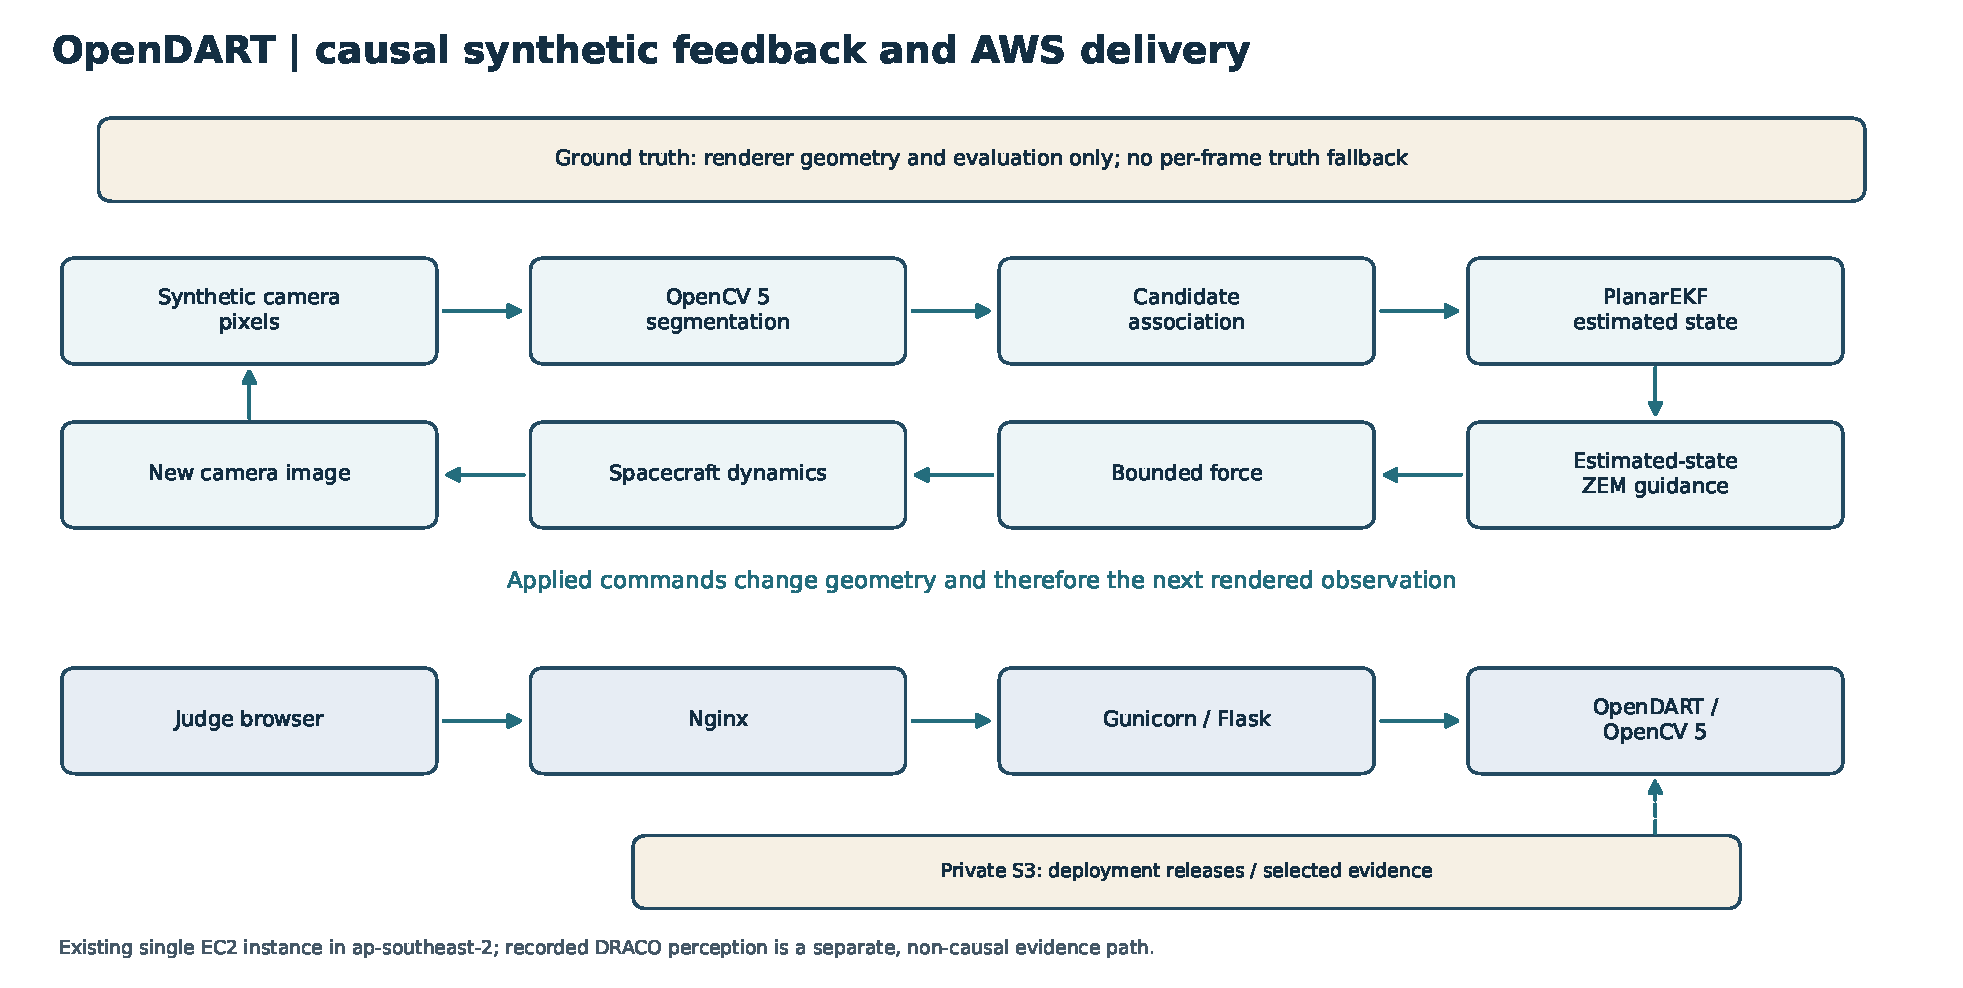
\includegraphics[width=\linewidth]{images/overall_system.pdf}
\caption{Implemented synthetic causal loop and existing AWS delivery. Ground truth supplies geometry to rendering and evaluation only; guidance uses the estimate. S3 stores private deployment releases and selected evidence.}\label{fig:system}
\end{figure}

\subsection{OpenCV 5: pixels to an estimator measurement}
Figure~\ref{fig:camera} shows a detection example. The detector receives image arrays rather than target coordinates. Its frozen path normalises finite intensity values, applies a $3\times3$ Gaussian filter, thresholds relative to a robust background estimate, performs morphological opening and extracts connected components. OpenCV measures component area, intensity-weighted centroid, apparent area radius and contour descriptors. A covariance floor represents localisation/illumination uncertainty; it is not a guarantee of calibrated state uncertainty.

Association uses image continuity and an estimated projection/size prior where supplied, with explicit acquisition, loss and reacquisition. It is an image-space target hypothesis rather than learned semantic body recognition. The selected centroid and size enter navigation; no per-frame simulator identity or target position is substituted when detection fails. Truth is available to render the scene and score errors, while guidance receives estimated relative state. A bundled reference-image patch may texture the modelled disks; this changes appearance, not the causal environment into historical flight footage.

\begin{figure}[htbp]\centering
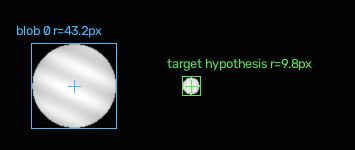
\includegraphics[width=.68\linewidth]{images/synthetic_camera_detail.png}
\caption{Display crop of the nominal camera result at 240~s; inference used the complete original frame. OpenCV extracts components and a target hypothesis from pixels. Labels describe image measurements, not privileged semantic truth.}\label{fig:camera}
\end{figure}

\subsection{Current PlanarEKF and monocular scale}
The current visual state is $x_p=[\rho_x,\rho_y,\nu_x,\nu_y]^T$, target minus spacecraft. For camera forward $f$, image right $q$, $Z=f^T\rho$, $X=q^T\rho$ and principal point $c_x$, the measurement prediction is
\[
h(x_p)=\begin{bmatrix} f_{\!x}X/Z+c_x \\ \log(f_{\!x}R/Z+b_r) \end{bmatrix},\qquad
R=88\ \mathrm{m},\quad b_r=1.07\ \mathrm{px}.
\]
The measured second component is the logarithm of the detector's area radius, not a direct range measurement. Known physical radius $R$ is an essential monocular scale assumption. The additive detector-radius offset $b_r$ predicts the measured extent: it was calibrated offline for this synthetic renderer/detector, \emph{not} for the DRACO instrument. Measurement variance and gating remain frozen; the size-variance floor is 0.10 in fractional/log-size terms. The planar image's fixed vertical centre does not supply an independent second bearing.

The EKF predicts using the applied bounded force and the existing physical environment, then updates from the selected image measurement. Telemetry distinguishes accepted updates, missing candidates/failed association, border clipping, invalid measurements/geometry, small components and innovation rejection. Missing images are not called NIS rejections. With no usable update the state is predicted only. Staleness beyond 5~s or excessive fractional range uncertainty inhibits thrust via NAV\_HOLD. The planar terminal-coast threshold is 12~s of estimated time to go, distinct from historical 3D coast settings. Camera pointing follows the estimate with the implemented rate limit; camera calibration/attitude knowledge is idealised.

\subsection{Agentic Vision and failure handling}
The operational sequence is OBSERVE $\rightarrow$ PERCEIVE $\rightarrow$ ESTIMATE $\rightarrow$ DECIDE $\rightarrow$ ACT $\rightarrow$ WORLD CHANGES $\rightarrow$ OBSERVE (Figure~\ref{fig:agentic}). No candidate or a blackout prevents a measurement update. Prolonged loss triggers NAV\_HOLD and zero thrust; new image evidence can reacquire the track and restore updates and guidance. Explicit terminal coast and opening-motion logic also command zero force. Reacquisition is not a hidden truth fallback.
\begin{figure}[htbp]\centering
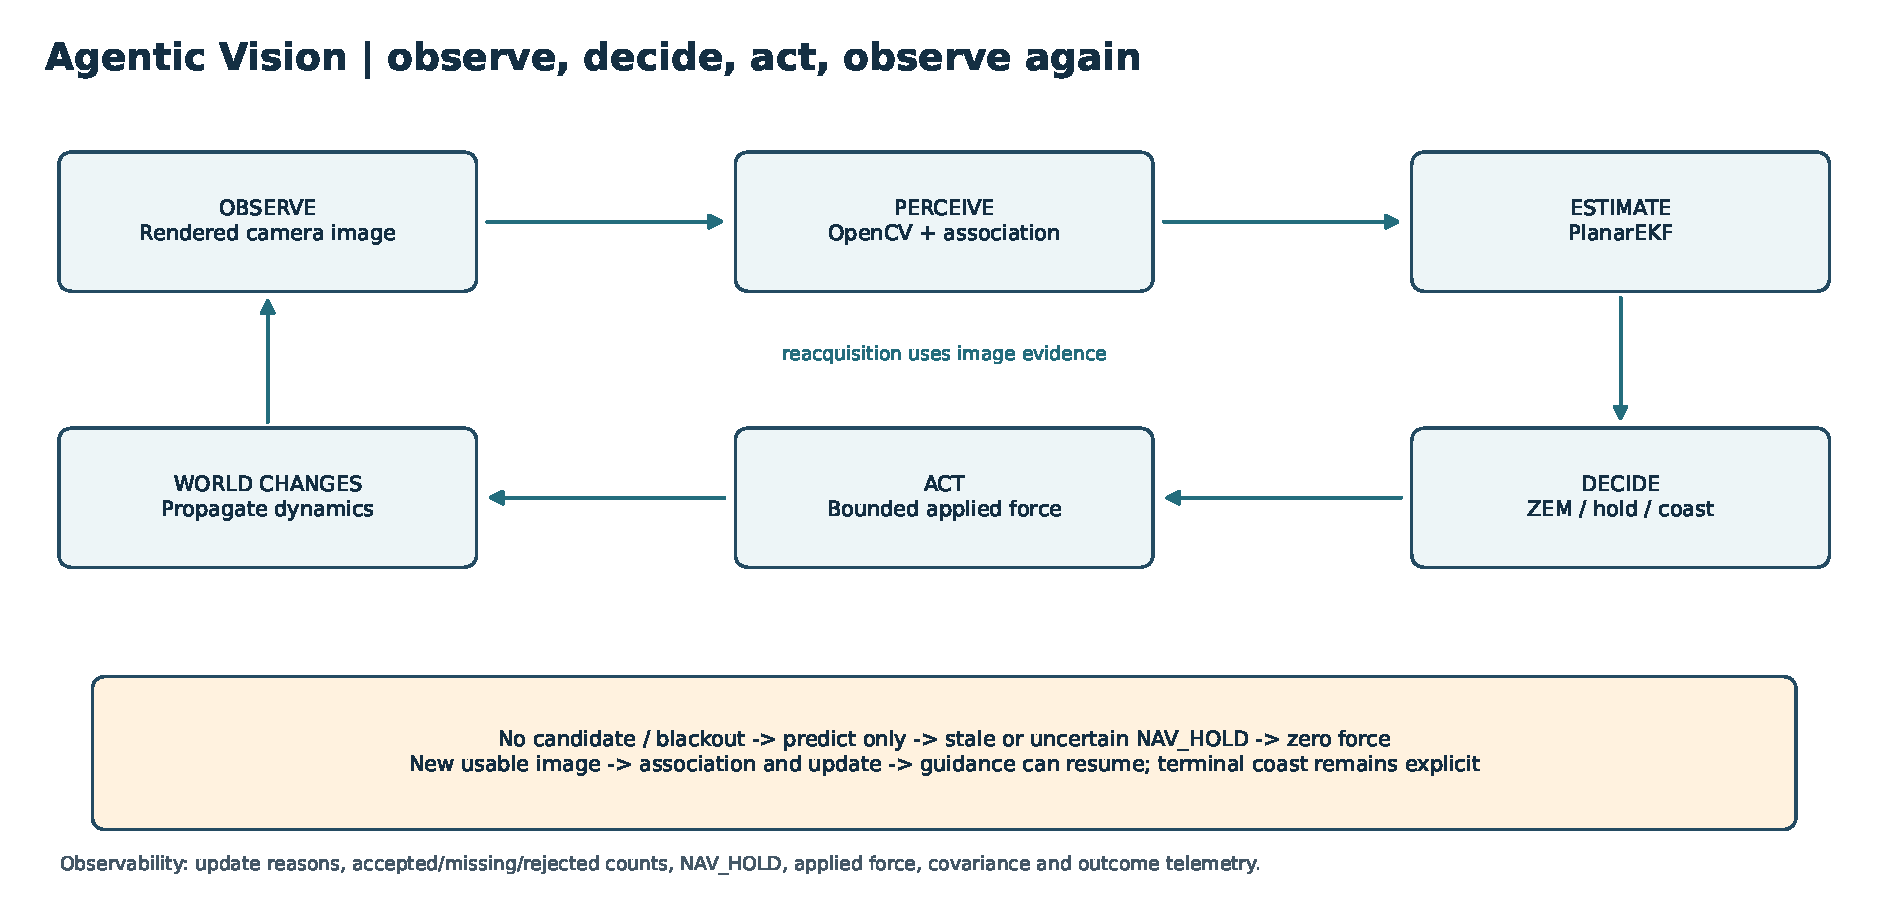
\includegraphics[width=\linewidth]{images/agentic_vision.pdf}
\caption{Implemented Agentic Vision workflow. Visual measurements change estimated state and subsequent action; applied action changes the next observation. Telemetry exposes loss, hold, coast and recovery.}\label{fig:agentic}
\end{figure}
\section{Supporting three-dimensional dynamics and control}
The following derivations preserve the partner's restricted-binary 3D model and controller treatment. The fast approach, optical-bearing experiment, 11.92~h surrogate orbit and 5~s/8~s coast choices in this section are historical/supporting settings, not the primary competition scenario. The planar simulation embeds its XY state in the existing environment, but uses the distinct camera, initial geometry, 42900~s orbit and 12~s estimated-coast setting described above. Guidance has not been redesigned during Tasks 1--3A.6.
\subsection{Parameter selection and consistency}
The default binary is a clearly labelled, pre-impact-like circular surrogate. It uses a 1190~m centre separation, an 11.92~h period and secondary mass fraction 0.00925. The total gravitational parameter is derived from these choices, rather than independently specifying a contradictory mass.
\[ n = \frac{2\pi}{T}, \quad \mu_{\mathrm{tot}} = n^{2}a^{3}, \quad \eta = \frac{\mu_{2}}{\mu_{\mathrm{tot}}} \]
The resulting $n$ is $1.4642023926 \times 10^{-4}\mathrm{~rad/s}$, total GM is $36.127932477\mathrm{~m^3/s^2}$ and binary relative orbital speed is $0.174240085\mathrm{~m/s}$.

\begin{table}[h]
\centering
\resizebox{\linewidth}{!}{\begin{tabular}{lll}
\toprule
\textbf{Quantity} & \textbf{Default} & \textbf{Provenance and interpretation} \\
\midrule
Binary separation $a$ & 1190 m & Simplified value from Ref.~\cite{voyatzis}, Table 1 \\
Binary period $T$ & 42912 s = 11.92 h & Pre-impact value in Refs.~\cite{voyatzis,ernst}; rounded surrogate \\
Secondary fraction $\eta$ & 0.00925 & Nominal normalised value in V; adopted model \\
Total GM & 36.127932477 m$^3$/s$^2$ & Derived from $a$ and $T$ \\
Didymos surface semi-axes & 425, 424, 310 m & Ref.~\cite{voyatzis} physical-size approx: geometry only \\
Dimorphos surface semi-axes & 88, 87, 58 m & Ref.~\cite{voyatzis} physical-size approx: geometry only \\
Didymos spin period & 8136 s = 2.26 h & Refs.~\cite{voyatzis,bigot}; fixed spin axis \\
Sun position & (1.5 AU, 0, 0) & Chosen fixed short-arc geometry \\
Reflectivity coefficient $C_R$ & 1.5 & Chosen cannonball assumption \\
Effective illuminated area & 5 m$^2$ & Chosen spacecraft assumption \\
Initial / dry spacecraft mass & 500 / 480 kg & Experiment settings; not actual hardware \\
Maximum resultant force & 10 N & Ideal actuator experiment setting \\
Specific impulse & 220 s & Experiment setting \\
Fast/slow closing speed & 6100 / 10 m/s & Impact-like / educational test regimes \\
Guidance interval & 1 s & Chosen sampled controller rate \\
\bottomrule
\end{tabular}}
\end{table}

The table in Ref.~\cite{voyatzis} quotes masses $5.32 \times 10^{11}$ and $4.94 \times 10^{9}$~kg and a period of 11.37~h. With $G = 6.67430 \times 10^{-11}$~SI and $a = 1190$~m, those masses yield $GM = 35.83698642\mathrm{~m^3/s^2}$ and a point-mass Kepler period of about 11.9683~h. Conversely, 11.37~h at that separation implies $GM = 39.70769616\mathrm{~m^3/s^2}$ in the point-mass model. Extended-body orbital corrections can matter, but the table must not be silently used as an exactly consistent point-mass parameter set. Some normalised dimensions also differ from directly dividing the physical dimensions by the stated separation.

The chosen geometric ellipsoids are illustrative fits, not registered modern shape meshes or fitted impact-era orientations. The model should be called ``Didymos-Dimorphos inspired'' until a coherent ephemeris/shape solution is installed. Do not change the period to the post-impact value while describing the same run as a reconstructed pre-impact approach.

\subsection{Frames, states and binary ephemeris}
Let I denote nonrotating axes centered on the binary barycenter. Strictly, the origin accelerates under external gravity; this is handled by indirect acceleration terms. Let B1 and B2 be asteroid body frames. Let C denote the camera frame in the supporting experiment. All vectors below are in I unless identified otherwise.

The code places the binary orbit in the I x-y plane. Its separation vector is:
\[ d(t) = a [\cos(nt+\phi_{0}), \sin(nt+\phi_{0}), 0]^T \]
\[ r_{1} = -\eta d \]
\[ r_{2} = (1-\eta)d \]
\[ a_{i} = -n^{2}r_{i} \]
Velocities are the exact time derivatives. These expressions preserve the barycenter and satisfy the circular two-point-mass relative equation with the derived GM.

The navigation state is target minus spacecraft:
\[ \rho = r_{t} - r_{s} \]
\[ \nu = v_{t} - v_{s} \]
\[ x = [\rho^{T}, \nu^{T}]^{T} \]
The spacecraft plant state is:
\[ y = [r_{s}^{T}, v_{s}^{T}, m]^{T} \]

This sign convention is important. A positive spacecraft acceleration in $x$ decreases the relative acceleration in $x$. Camera line of sight points along positive $\rho$, from the spacecraft toward the target.

The historical 3D default approach travels along positive I z, so initial $\rho$ has positive z and relative velocity $\nu$ has negative z. That makes the incoming spacecraft approach the target's negative-z side. It is a convenient spatial test and is not the momentum-optimal direction in the binary orbital plane.

\subsection{Translational dynamics and environmental forces}

\subsubsection{Spacecraft equation}
\[ \dot{r}_{s} = v_{s} \]
\[ \dot{v}_{s} = g_{b}(t, r_{s}) + a_{\mathrm{tide}}(r_{s}) + a_{\mathrm{SRP}}(t, r_{s}, m) + \frac{F}{m} \]
\[ g_{b}(t, r) = -\sum_{i=1}^{2} \mu_{i} \frac{r - r_{i}(t)}{|r - r_{i}(t)|^{3}} \]
The spacecraft does not perturb the binary before contact. Its mass is negligible relative to either body. Point-mass gravity is used only up to the finite contact surface, so the simulated trajectory never needs to pass through a gravitational centre.

\subsubsection{Solar tide}
Let $s$ be the barycenter-to-Sun vector:
\[ a_{\mathrm{tide}}(r) = \mu_{\odot} \left[ \frac{s - r}{|s - r|^{3}} - \frac{s}{|s|^{3}} \right] \]
The second term is essential: solar attraction of the barycenter is shared by the spacecraft and must be subtracted. For small displacement compared with solar distance:
\[ a_{\mathrm{tide}} \simeq \frac{\mu_{\odot}}{s^{3}} (3\hat{s}\hat{s}^{T} - I_{3})r \]
The implementation evaluates the exact difference using a numerically stable algebraic expression rather than subtracting nearly equal large forces. The Sun vector is fixed over the short simulated arc. The circular binary itself is prescribed and does not respond to solar tides; this is a restricted short-arc approximation, not a fully coupled Sun-binary integration.

\subsubsection{Solar radiation pressure}
\[ a_{\mathrm{SRP}} = -\chi P_{1\mathrm{AU}} C_{R} \frac{A}{m} \left( \frac{r_{1\mathrm{AU}}}{|s - r_{s}|} \right)^{2} \frac{s - r_{s}}{|s - r_{s}|} \]
Here $\chi$ is one in light and zero in hard umbra, $P_{1\mathrm{AU}}$ is $4.56 \times 10^{-6}\mathrm{~N/m^2}$ and $C_R$ is the effective radiation-pressure coefficient. The minus sign makes the force point away from the Sun. Do not use a solar flux in W/m$^2$ as a pressure without the appropriate division by light speed. Do not replace $C_R$ by $1+C_R$ when $C_R$ already represents the effective coefficient.

The default unshadowed SRP acceleration is about $3.04 \times 10^{-8}\mathrm{~m/s^2}$ at 500~kg and 1.5~AU. Its uncorrected constant-acceleration displacement over 600~s is about 5.5~mm. This small value for a short test does not contradict its importance for the multi-day orbits in Ref.~\cite{voyatzis}.

The shadow model intersects the spacecraft-to-Sun ray with both rotating ellipsoids. It neglects the finite solar disk, penumbra, spacecraft shape and attitude-dependent area. Switching is discontinuous at shadow boundaries. Use a smooth illumination model or shadow-transition events for precision long-arc SRP work.

\subsubsection{Mass, force and fuel}
\[ \dot{m} = -\frac{|F|}{I_{\mathrm{sp}} g_{0}} \]
\[ |F| \le F_{\mathrm{max}}, \quad m \ge m_{\mathrm{dry}} \]
At a controller update, the desired acceleration is converted to force using the current mass, clipped by resultant-force magnitude and clipped again by the remaining propellant budget over the next update interval. The applied force is held constant during that interval. Thus its acceleration increases slightly as mass falls. The EKF predictor receives this applied force.

The recorded delta-v is the scalar integral of thrust acceleration magnitude; for each constant-force segment it is computed from $I_{\mathrm{sp}} g_0 \ln(m_{\mathrm{start}}/m_{\mathrm{end}})$. It is not the norm of net inertial velocity change, which also contains gravity and directional cancellation.

This ideal omnidirectional resultant force models an already-closed inner attitude/actuator loop. It cannot establish feasibility for a real body-fixed thruster arrangement. There is no simulated torque, pointing-rate limit, plume constraint, minimum impulse bit or valve delay.

\subsection{Relative dynamics and linearisation}
Define the natural relative acceleration:
\[ d_{r}(t, x, m) = a_{t}(t) - g_{b}(t, r_{t} - \rho) - a_{\mathrm{tide}}(r_{t} - \rho) - a_{\mathrm{SRP}}(t, r_{t} - \rho, m) \]
Then:
\[ \dot{\rho} = \nu \]
\[ \dot{\nu} = d_{r} - u \]
\[ u = \frac{F}{m} \]

The target acceleration comes from differentiating the prescribed target ephemeris. Do not calculate it by inserting the target centre into a field containing its own point mass; that produces a self-gravity singularity. If a future target ephemeris already includes perturbations, do not add those perturbations to its acceleration again.

Ignoring mass as an estimated state, the local state matrix and control matrix are:
\[ A = \begin{bmatrix} 0 & I_{3} \\ G_b & 0 \end{bmatrix}, \quad B = \begin{bmatrix} 0 \\ -I_{3} \end{bmatrix} \]
For point gravity, with $\delta_{i} = r_{s} - r_{i}$:
\[ G_{b} = \sum_{i} \mu_{i} \left[ \frac{3 \delta_{i} \delta_{i}^{T}}{|\delta_{i}|^{5}} - \frac{I_{3}}{|\delta_{i}|^{3}} \right] \]
$G_b$ is positive the spacecraft field's spatial Jacobian, not its negative: differentiating $-g(r_t - \rho)$ introduces two minus signs. The code includes an analytic point-gravity gradient for verification and central differences of the complete relative drift for EKF linearisation. This derivative is only locally meaningful away from a hard shadow boundary.

Under a frozen double-integrator approximation, the sampled matrices are:
\[ \Phi = \begin{bmatrix} I_{3} & \Delta t I_{3} \\ 0 & I_{3} \end{bmatrix}, \quad \Gamma = \begin{bmatrix} -\frac{1}{2} \Delta t^{2} I_{3} \\ -\Delta t I_{3} \end{bmatrix} \]
That model is useful for a first controller calculation. It should not replace integration of the two-body force field in every experiment, especially the slow laboratory case.

\subsection{Connection to rotating-frame models}
Let $R$ map rotating binary coordinates into I, and let $\omega = (0, 0, n)^T$. The coordinate conversion includes velocity transport:
\[ r_{I} = R r_{R} \]
\[ v_{I} = R (v_{R} + \omega \times r_{R}) \]
\[ \dot{v}_{R} = R^{T} a_{I} - 2\omega \times v_{R} - \omega \times (\omega \times r_{R}) \]

This yields the familiar x Coriolis term $+2n \dot{y}$, y Coriolis term $-2n \dot{x}$, and outward $n^{2}x / n^{2}y$ centrifugal terms. There is no centrifugal term along z. The delivered dynamics integrate nonrotating axes, so these fictitious accelerations must not also be added there.

Using distance unit $a$ and time unit $1/n$ gives the dimensionless CR3BP form when gravity is point mass and no Sun, SRP or control is present. A dimensioned Jacobi integral for that restricted case is:
\[ C = n^{2}(x_{R}^{2} + y_{R}^{2}) + 2\sum_{i} \frac{\mu_{i}}{r_{i}} - |v_{R}|^{2} \]
The tests check its numerical conservation in the appropriate unforced model. With thrust, solar perturbations or rotating nonspherical gravity, the same expression is generally not conserved. Conservation of inertial spacecraft two-body energy is also not the correct test in a time-dependent binary potential.

\subsection{Two simple feedback controllers}

\subsubsection{PD tracking of an intercepting reference}
Choose a desired constant closing speed $V$ and nominal centre-passage time $t_f$. In the default approach direction $e_z$:
\[ \rho_{\mathrm{ref}} = V(t_{f} - t) e_{z}, \quad \nu_{\mathrm{ref}} = -V e_{z} \]
Let $e = \rho - \rho_{\mathrm{ref}}$ and $\dot{e} = \nu - \nu_{\mathrm{ref}}$. Request spacecraft acceleration:
\[ u_{\mathrm{PD}} = \hat{d}_{r} + \omega_{n}^{2} e + 2\zeta \omega_{n} \dot{e} \]
With exact state/drift, continuous actuation, no saturation and zero reference second derivative:
\[ \ddot{e} + 2\zeta \omega_{n} \dot{e} + \omega_{n}^{2} e = 0 \]
Positive natural frequency and damping ratio give exponentially stable tracking error in this idealised regime. For a general accelerating reference, subtract its second derivative in the command. The implemented reference is linear, so that term is zero.

The delivered tuned PD uses $\zeta = 1$ and natural frequency $0.012\mathrm{~rad/s}$. Gains are $k_p = 1.44 \times 10^{-4}\mathrm{~s^{-2}}$ and $k_d = 0.024\mathrm{~s^{-1}}$. Initial requested transverse acceleration exceeds the $0.02\mathrm{~m/s^2}$ actuator limit, so the actual early error dynamics do not obey the unsaturated proof. The initial lower choice 0.008~rad/s misses in the fast example. Both outcomes are retained to expose gain and saturation effects.

Tracking a linearly closing reference is different from regulating $\rho$ and $\nu$ to zero. The latter would deliberately brake toward rendezvous. Surface contact occurs before the reference reaches the target centre.

\subsubsection{ZEM feedback: the recommended interception baseline}
For a closing estimate, compute a straight-line time to closest approach:
\[ \tau = -\frac{\rho^{T} \nu}{\nu^{T} \nu} \]
A nonpositive $\tau$ indicates opening motion and commands zero thrust in this demonstrator. With locally constant natural relative acceleration:
\[ Z = \rho + \tau \nu + \frac{1}{2} \tau^{2} \hat{d}_{r} \]
$Z$ is the predicted zero-control displacement from the target centre at the frozen terminal time. The applied request is:
\[ u_{\mathrm{ZEM}} = \frac{3Z}{\tau^{2}} \]
Derivation: for fixed positive $\tau$ and constant drift, the terminal-position constraint is:
\[ 0 = Z - \int_{0}^{\tau} (\tau - s) u(s) ds \]
Minimizing one-half the integral of squared acceleration subject to this constraint and free terminal velocity gives:
\[ u(s) = \frac{3(\tau - s)}{\tau^{3}} Z \]
The value at $s=0$ is the commanded $3Z/\tau^{2}$. A constant-acceleration endpoint correction would instead have coefficient 2; these are different optimization assumptions. The delivered law repeatedly recalculates the estimate, drift and $\tau$, so it is a receding feedback law rather than one open-loop polynomial.

This derivation does not prove constrained interception with errors, saturation, dropouts or strongly varying gravity. $\tau$ is an approximate time-to-go, not an exact gravity-aware intercept solution. The example results and tests establish behavior for the supplied cases. For large curvature, replace the local $Z$ estimate with a propagated zero-control trajectory and a state-transition sensitivity or solve a constrained predictive guidance problem.

The code floors the denominator at a two-second time-to-go and uses a five-second terminal coast by default. The coast avoids commanding rapidly changing corrections from a vanishing horizon or an invalid full-object centroid. The slow case uses eight seconds. These are design settings to sweep, not mission requirements.

Atchison's proportional-navigation concept could also be compared using the LOS angular rate. It is not implemented in this package. ZEM is chosen here because it exposes predicted miss and interfaces directly with a position/velocity estimate.

\subsubsection{Reachability before tuning}
With free terminal transverse velocity, a rough necessary bound on a correctable transverse displacement is:
\[ |Z_{\perp}| \le \frac{1}{2} a_{\mathrm{max}} \tau^{2} \]
At $0.02\mathrm{~m/s^2}$ and 600~s this is about 3600~m, before fuel, pointing or other constraints. At 60~s it is only 36~m. The same gain settings cannot recover arbitrary late detection errors. The unconstrained minimum-energy law's initial acceleration is $3Z/\tau^{2}$, so its no-initial-saturation envelope is smaller than the simple reachability bound.

\subsection{Surface contact, impact measurements and numerics}
For each body, transform the spacecraft displacement into its body frame. Let $b_{i} = Q_{i}(t)^{T} (r_{s} - r_{i})$, with geometric semi-axes $a_i$, $b_i$, $c_i$. Define:
\[ g_{i}(t) = \frac{b_{ix}^{2}}{a_{i}^{2}} + \frac{b_{iy}^{2}}{b_{i}^{2}} + \frac{b_{iz}^{2}}{c_{i}^{2}} - 1 \]
An inward crossing of zero is surface contact. Both bodies have terminal events. Contact with the selected target is \texttt{TARGET\_IMPACT}; contact with the other body is \texttt{WRONG\_BODY\_IMPACT}. If the target range reaches a local minimum before contact, the experiment terminates as \texttt{MISS}. A duration limit gives \texttt{TIMEOUT}. These are terminal-approach semantics, not an exhaustive classification of a long, looping trajectory.

At 6100~m/s, crossing the target's 116~m polar diameter takes only about 0.019~s. Checking distance at 1~Hz can miss the entire body. Even an event-aware ODE solver can miss two surface crossings inside one large step if both endpoints are outside.

The simulator therefore separates the one-second command update from internal integration. Before a possible encounter during an interval, it limits the internal step using a quarter of the body's smallest semi-axis divided by a conservative relative-speed estimate. DOP853 then localizes the inward event. Tests deliberately send a fast trajectory through a body with both nominal interval endpoints outside. Both primary and secondary contacts are detected.

The speed bound and step policy are designed for these terminal scenarios; they are not a formal collision-detection guarantee for every possible high-acceleration trajectory. Extend the strategy with swept-volume/continuous collision checks when introducing new regimes or complex meshes.

At contact, normal incidence is evaluated using the ellipsoid normal and spacecraft velocity relative to the rotating surface:
\[ v_{\mathrm{surf}} = v_{t} + \omega_{t} \times (r_{s} - r_{t}) \]
The angle is zero for inward motion along the negative outward normal. No post-contact dynamics are integrated.

Metrics must be named precisely. The target-centre distance at contact is about the local surface radius; it should not be reported as a miss. For nonimpacting cases, the centre distance at the first closest approach is the geometric miss metric. The reported transverse distance is in the initial I x-y impact plane and is not a terrain-referenced surface aiming error or a fully reconstructed B-plane coordinate.

\section{Historical supporting 3D camera and BearingEKF}
This section retains the older geometric-bearing experiment. Unlike the delivered planar visual path, its observations are projected synthetic measurements rather than detections from rendered pixels. Its absence of a known-size measurement must not be transferred to the current PlanarEKF description.

The ideal camera uses a right-handed OpenCV-style frame: x right, y down, z forward. Let $R_{CI}$ map I to C:
\[ p_{C} = R_{CI} \rho = [X, Y, Z]^{T} \]
\[ u = f_{x} \frac{X}{Z} + c_{x}, \quad v = f_{y} \frac{Y}{Z} + c_{y}, \quad Z > 0 \]
The measurement Jacobian is:
\[ H = \begin{bmatrix} f_{x}/Z & 0 & -f_{x}X/Z^{2} \\ 0 & f_{y}/Z & -f_{y}Y/Z^{2} \end{bmatrix} R_{CI} \]
Scaling $\rho$ by any positive factor leaves the ideal pixel unchanged. The radial direction is in the instantaneous measurement Jacobian's null space. With unforced constant-velocity relative motion, a scale transformation of both $\rho$ and $\nu$ preserves the whole bearing history. A single image does not supply range or range rate.

Known observer acceleration can break that ambiguity in suitable geometries, but closing motion alone and noisy small corrections do not guarantee useful range observability. A coarse prior and covariance monitoring are essential. Known target size is a possible additional measurement with shape, illumination and resolution uncertainty; it is not part of this historical BearingEKF.

The EKF predicts the nonlinear six-state dynamics using applied force and known mass. Its covariance propagation uses a locally frozen A, a matrix exponential and a Van Loan process-noise integral. Acceleration spectral density has units m$^2$/s$^3$. The model assumes exact target ephemeris, known camera attitude and known applied control.

For pixel residual $y$, covariance $R$ and innovation covariance $S$:
\[ S = H P^{-} H^{T} + R, \quad K = P^{-} H^{T} S^{-1} \]
\[ \hat{x}^{+} = \hat{x}^{-} + K y \]
\[ P^{+} = (I - KH) P^{-} (I - KH)^{T} + K R K^{T} \]
The Joseph covariance form reduces numerical loss of symmetry/positive definiteness. The two-dimensional normalised innovation squared is gated at 9.21034, the approximate 99\% chi-square threshold under the assumed Gaussian model. A confidence score is not automatically a valid pixel covariance; it must be calibrated from localization residuals.

The experiment inhibits guidance if accepted observations become stale, predicted transverse uncertainty becomes too large or fractional range uncertainty exceeds its configured bound. This \texttt{NAV\_HOLD} behavior sacrifices correction authority when information is inadequate. It is an explicit demonstration policy, not a complete autonomy or safety system.

The synthetic observation uses a point at the target centre, Gaussian pixel noise, a known target identity, independent random dropouts and a scheduled 200-220~s blackout. Camera pointing is computed from the estimated LOS with an instantaneous ideal attitude servo, not from the true LOS, preventing a silent fallback to truth feedback.

Ground truth is used only to generate observations and evaluate the run. There is no photometric rendering, centre-of-light bias, distractor population, optical occultation renderer, attitude estimation error or image-processing latency.

\section{Synthetic visual evaluation}
\subsection{Task 1: detector-size measurement calibration}
An offline synthetic renderer/detector calibration identified an approximately $+1.07$~px extent offset. Updating the measurement prediction reduced the seed-7 nominal errors in Table~\ref{tab:calibration}. This was a size-measurement bias correction, not covariance inflation or a controller redesign. Both before/after cases reached contact; impact alone concealed the earlier navigation error.
\begin{table}[htbp]\centering
\caption{Task 1 nominal comparison.}\label{tab:calibration}
\begin{tabular}{lrr}\toprule
Measure & Before & Calibrated \\\midrule
Final position estimation error (m) & 59.18 & 9.23 \\
Peak sampled position error (m) & 2096.93 & 375.07 \\
Maximum $|$range error$/\sigma|$ & 18.11 & 2.62 \\
Detector-radius offset (px) & 0 & 1.07 \\\bottomrule
\end{tabular}
\end{table}

\subsection{Task 2: bounded campaign and causal controls}
The main campaign crossed two appearances (analytic and bundled reference patches), seeds 0--11, and four conditions: nominal; image degradation (3~DN noise and 0.10 random dropout); a 40~s extended blackout at $[200,240)$~s; and an initial range-prior perturbation of $\pm1200$~m, with sign paired to seed parity. Other conditions retained the nominal $[200,220)$~s blackout. True initial geometry was held fixed across matched conditions; an altered estimate could legitimately alter pointing and subsequent motion.

Table~\ref{tab:campaign} summarises the main cells. All \textbf{96/96 guided cases reached TARGET\_IMPACT} within the tested bounded synthetic conditions, with no wrong-body impact, miss or timeout. Each of the eight appearance/condition cells is 12/12, with Wilson 95\% interval approximately $[0.758,1.000]$. Matched appearances/conditions are paired, so these are not 96 independent samples of general reliability. Temporally correlated frames are not binomial trials. The result is not ``100\% reliable'' flight performance. Final position error across the guided campaign was 7.78--12.19~m; this is estimation error, not residual miss distance at surface contact.

\begin{table}[htbp]\centering
\caption{Each row contains 12 seeds per appearance. Controls are excluded from guided totals.}\label{tab:campaign}
\begin{tabular}{lccc}\toprule
Condition & Analytic & Reference & Per-cell Wilson 95\% \\\midrule
Nominal & 12/12 contact & 12/12 contact & $[0.758,1.000]$ \\
Degraded image & 12/12 contact & 12/12 contact & $[0.758,1.000]$ \\
Extended blackout & 12/12 contact & 12/12 contact & $[0.758,1.000]$ \\
Range-prior error & 12/12 contact & 12/12 contact & $[0.758,1.000]$ \\\bottomrule
\end{tabular}
\end{table}

Four separate negative controls (both appearances, seed~7) all missed: BALLISTIC retained image updates but disabled actuation; NO\_MEASUREMENT supplied no accepted updates and commanded zero force. All four zero-thrust cases had closest target-centre approach approximately 615.52~m. No-measurement final estimation error was 446.44~m, compared with roughly 9--10~m in the analytic image-informed seed-7 examples. Matched image-feedback guidance changed the outcome from a miss to contact, with approximately 1.60~m/s analytic correction. This supports the causal architecture under the stated prior/size/scene assumptions.

During the extended blackout every tested run resumed an accepted update at 240~s and still reached contact. Median NAV\_HOLD was 35~s rather than nominal 15~s. Figure~\ref{fig:blackout} retains the offline recovery evidence; isolated missing frames and REACQUIRED counts should not be confused with distinct prolonged-loss episodes.
\begin{figure}[htbp]\centering
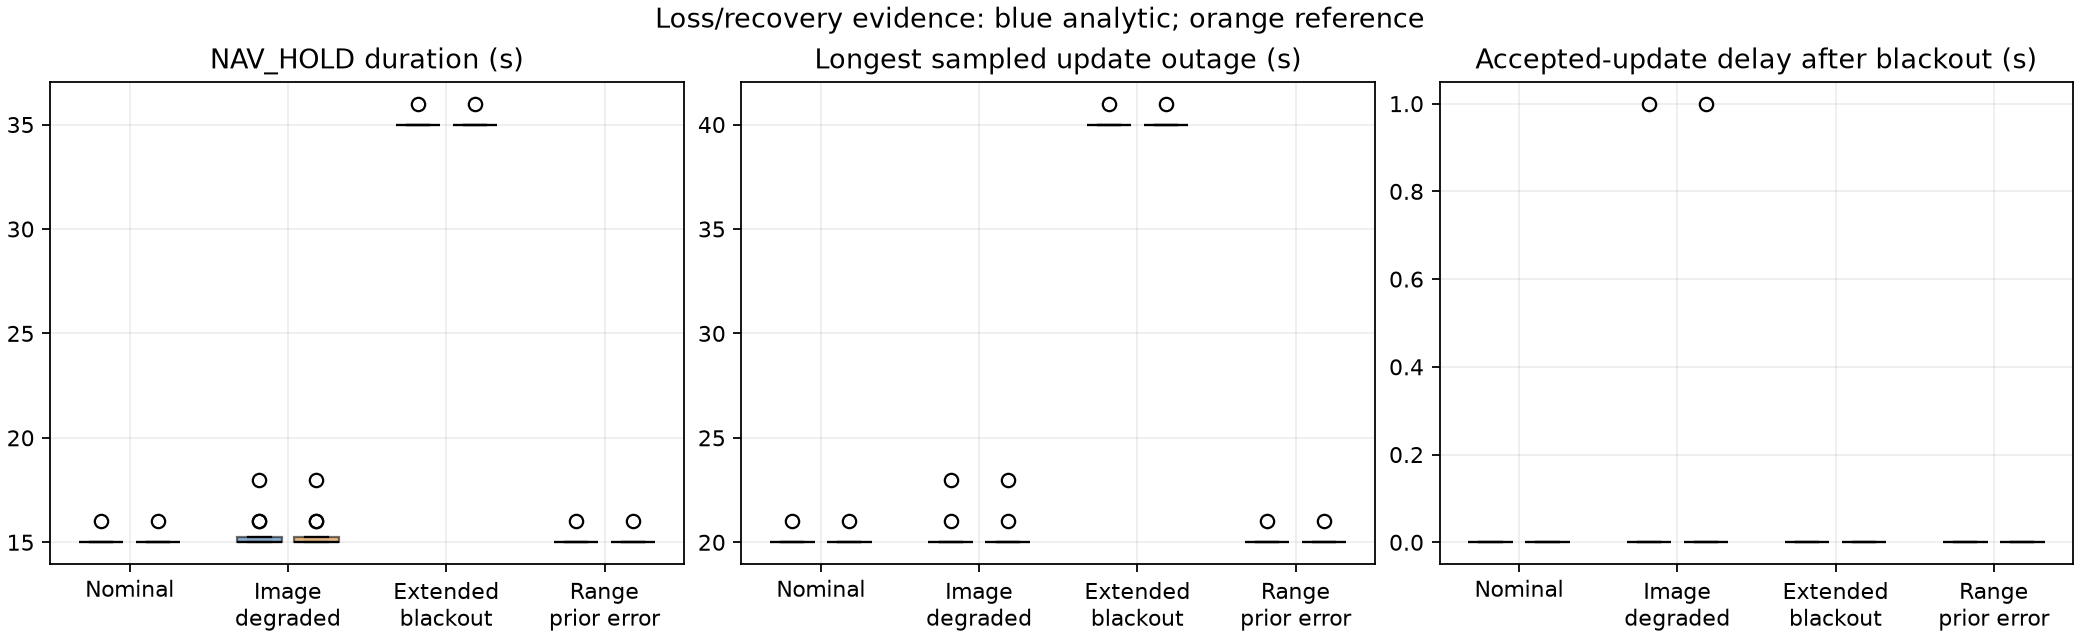
\includegraphics[width=\linewidth]{images/campaign_blackout.png}
\caption{Task 2 loss/recovery statistics. The extended-blackout condition lasts 40~s; sampled availability, hold and reacquisition remain distinct counters.}\label{fig:blackout}
\end{figure}

\subsection{Uncertainty and known-size sensitivity}
Useful navigation/control performance does not establish statistical EKF consistency. The campaign showed material \textbf{full-state covariance undercoverage} (Figure~\ref{fig:uncertainty}). Median per-run nominal full-state 95\% ellipsoid coverage was only 27.2\% (analytic) and 20.6\% (reference), despite much higher position-ellipse coverage. Nominal range-band coverage was 81.2\% and 73.5\%. At 500 and 580~s none of the 12 nominal full-state ellipsoids contained truth for either appearance. NIS remained below the update gate; low residuals therefore did not certify calibrated state uncertainty. These correlated-frame diagnostics are descriptive, not independent-trial coverage estimates.
\begin{figure}[htbp]\centering
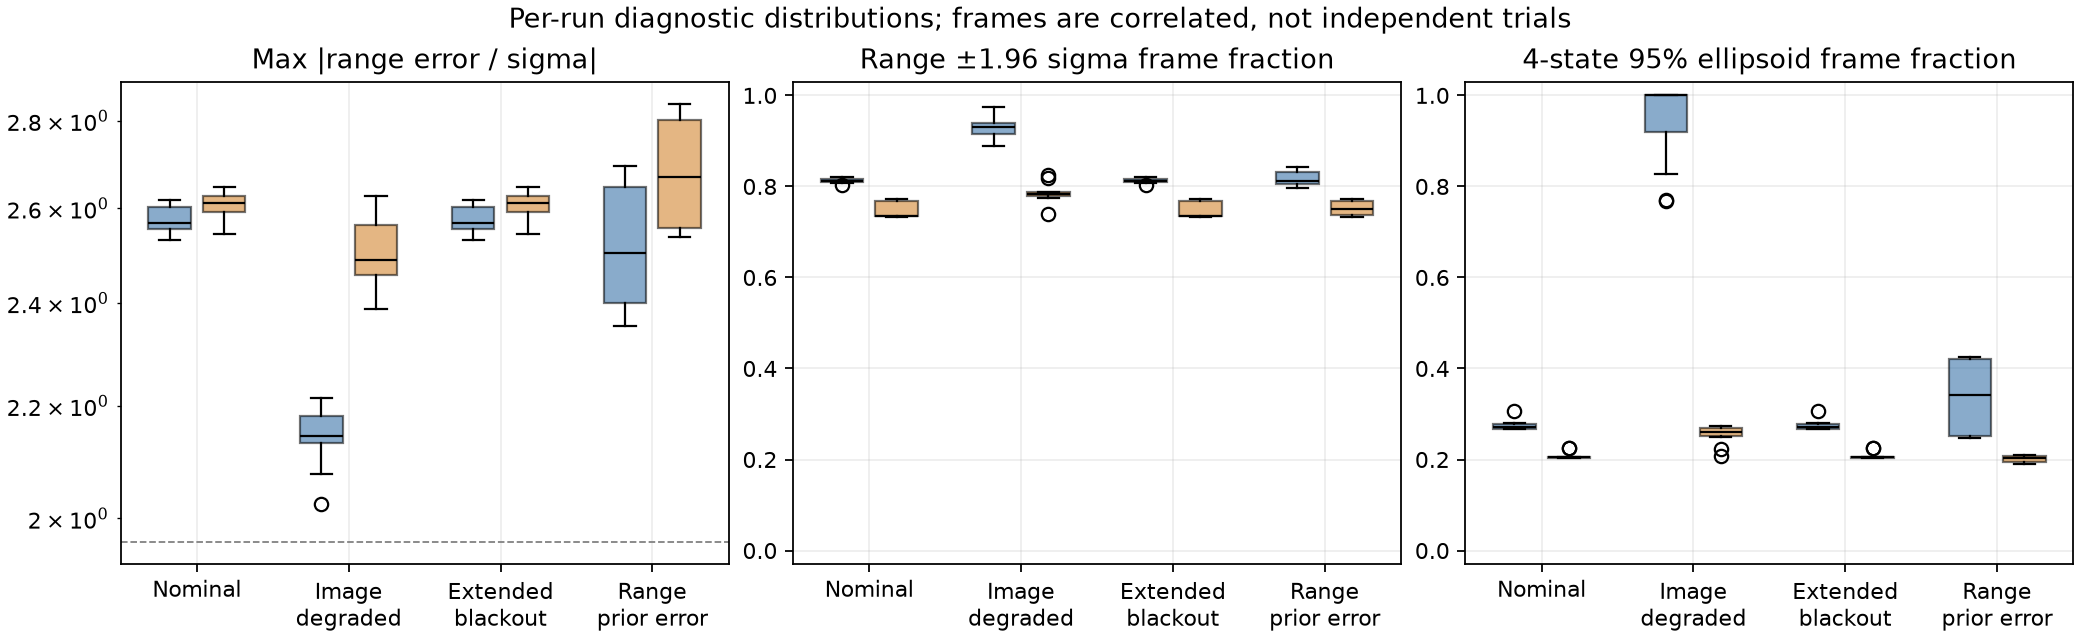
\includegraphics[width=\linewidth]{images/campaign_uncertainty.png}
\caption{Uncertainty diagnostics: useful contact outcomes coexist with substantial covariance undercoverage. Frame fractions are descriptive; blue denotes analytic appearance and orange reference appearance.}\label{fig:uncertainty}
\end{figure}

Ten separate seed-7 diagnostics varied only navigation's assumed radius by $\pm5\%$ and $\pm10\%$, keeping rendered radius, contact geometry, detector calibration and controller fixed. All reached contact, yet a reference $+10\%$ radius case had about 1615~m transient peak error and maximum normalised range error 9.46, despite only 4.33~m final error. Analytic $-10\%$ radius produced about 1426~m peak error and 10.85 maximum normalised range error. Final contact or accidental bias cancellation must not hide this monocular-scale sensitivity. These diagnostics are excluded from the 96-run guided success count and do not motivate further tuning in this frozen work.
\section{Real DRACO imagery: recorded perception evidence}
\subsection{Data and the frozen transfer baseline}
The local dataset contains 4000 calibrated PNG products with matching PDS4 XML labels from the official PDS Small Bodies Node \cite{pds} DRACO v3.0 \texttt{data\_dracocal} archive: terminal-phase acquisition from 22:00 to before 23:10 UTC and final-phase imagery from 23:10 UTC towards impact on 26 September 2022. The first acquisition is 22:00:00.446 and last is 23:14:23.328 UTC; the approximate impact reference is 23:14:24.183 UTC. XML-derived acquisition time orders the products; filename clocks are not substituted for those timestamps. Original images are $1024\times1024$ uint8 greyscale PNGs. No FITS processing is required. Stored PNG orientation is retained, with the archive's display convention documented.

Figure~\ref{fig:draco} shows representative progression. These are \textbf{prerecorded spacecraft images}. New control commands cannot alter their future frames. They test real-image perception/tracking only, not causal guidance or reconstruction of the flown navigation stack. The original synthetic detector produced components broadly, but its selected-target association did not transfer reliably; component availability must not be described as successful Dimorphos tracking.

\begin{figure}[htbp]\centering
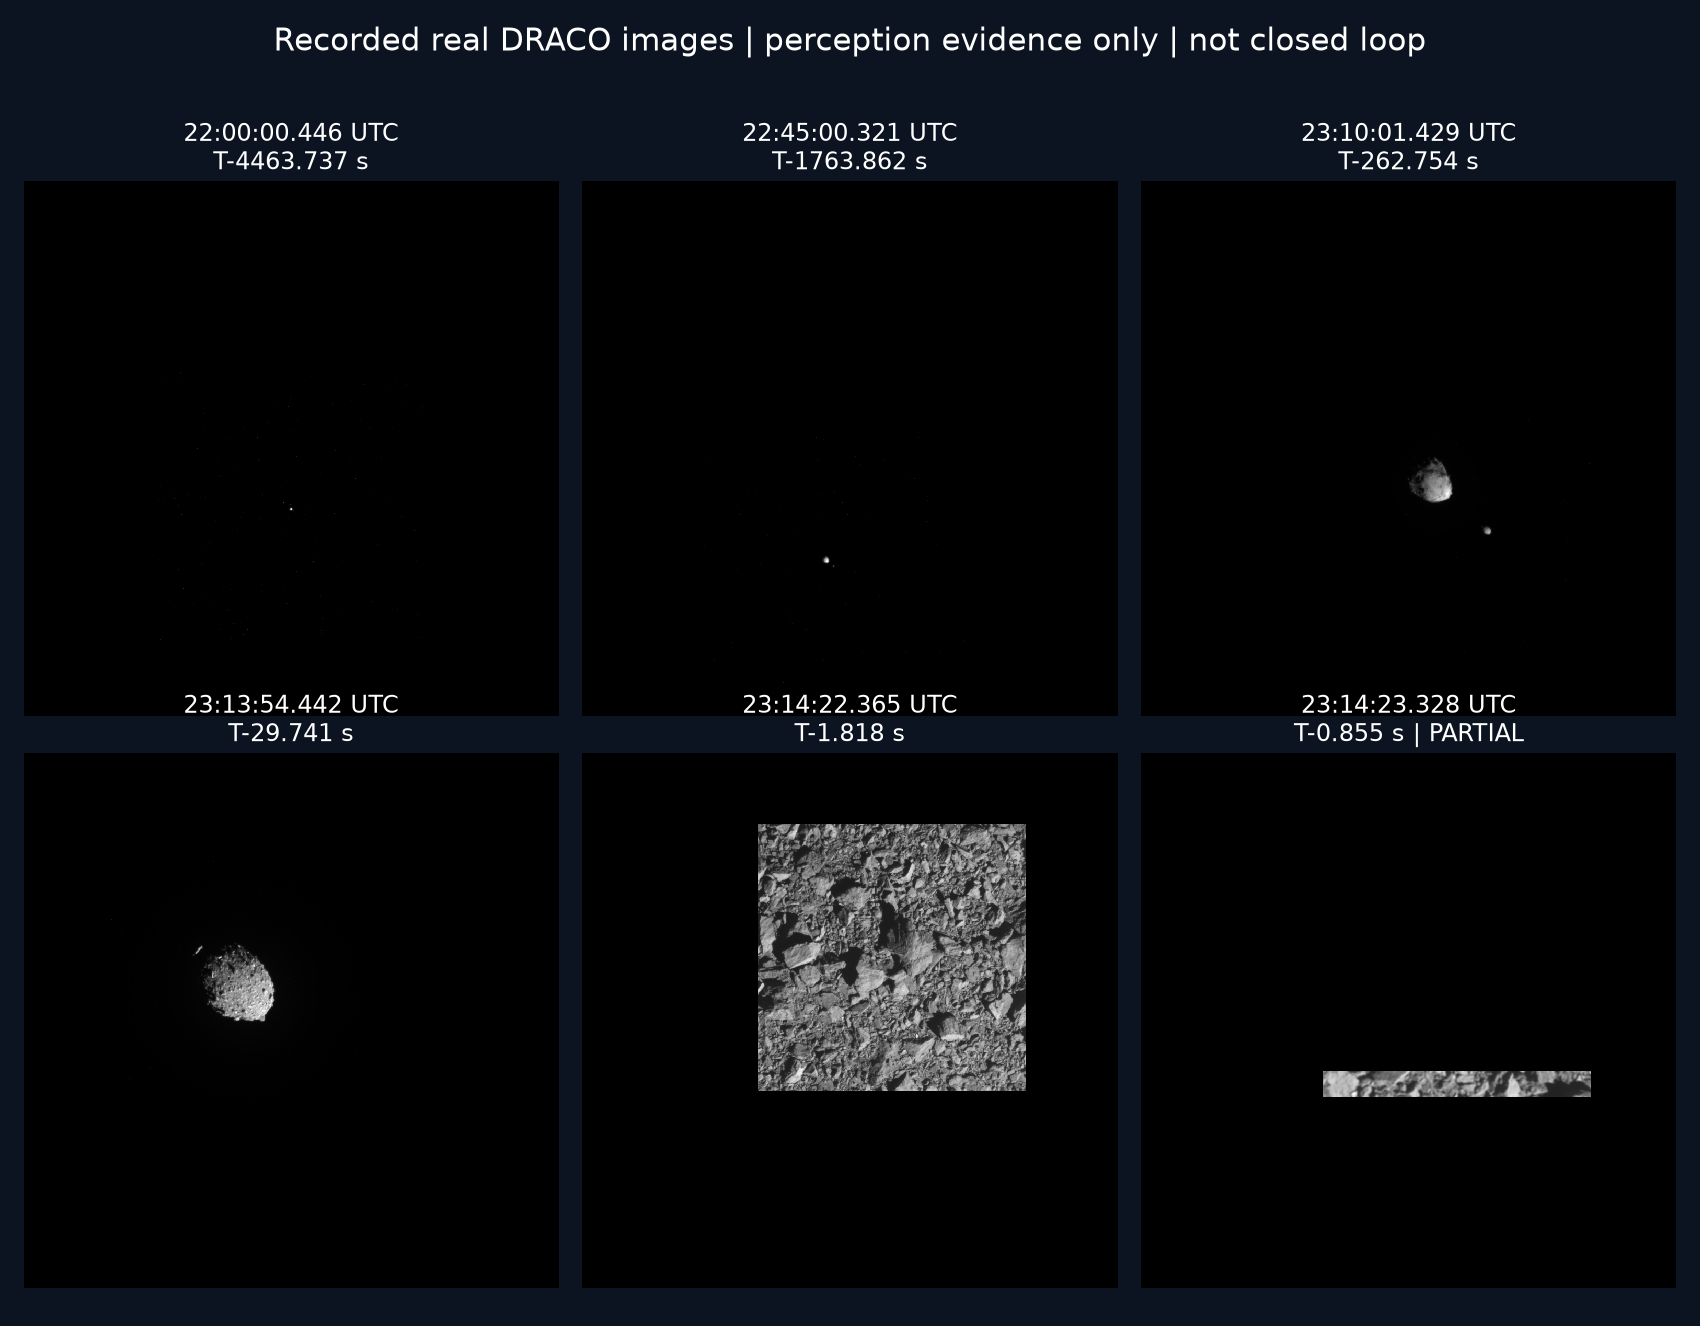
\includegraphics[width=.8\linewidth]{images/draco_progression.png}
\caption{Presentation-only contact sheet of curated original DRACO images with preserved XML-derived UTC. Early imagery is faint; late terrain is resolved; the last transmission is only a strip. No missing extent or target truth is inferred.}\label{fig:draco}
\end{figure}

\subsection{DRACO-specific perception method}
The separate, non-learned perception path uses causal past-only occupancy/persistence handling, OpenCV phase-correlation image translation, image-space acquisition/tracking, explicit loss/reacquisition and a resolved-foreground representation. It receives no synthetic truth, EKF state or guidance input. A unique separated smaller-body hypothesis must be confirmed over consecutive frames; its identity remains an image hypothesis. Significant resolved fragments are represented by a coarse visible-region envelope, not an invented physical centre or range. PARTIAL\_FRAME reports only transmitted content.

Optional operator-assisted tracking uses one fixed reviewed \emph{development} frame at 23:11:08.829 UTC and no later manual correction. Source/configuration and temporal rules were frozen before the final held-out scoring. No learned model or post-evaluation retuning was introduced. The 4000-frame replay is historical perception evidence, including unreviewed qualitative frames, not 4000 ground-truth-verified identifications.

\subsection{Real-image held-out benchmark}
Figure~\ref{fig:heldout} and Table~\ref{tab:draco} summarise the benchmark. Of 20 sampled held-out frames, 18 were reviewed: eight compact labels, eight visible-region labels and two uncertain labels. Two boundary-clipped cases remained UNREVIEWED and were excluded, not scored as negatives, failures, partial frames or zero IoU. No reviewed held-out labels occur in the final ten seconds. The final complete and partial examples are qualitative analysis cases outside this ordinary benchmark.
\begin{table}[htbp]\centering
\caption{Held-out comparison. Available-point medians are conditional on selection.}\label{tab:draco}
\begin{tabular}{lcc}\toprule
Measure & Original baseline & DRACO autonomous \\\midrule
Compact point within 5 px & 2/8 & 6/8 \\
Median available point error & 82.483 px ($n=6$) & 1.218 px ($n=6$) \\
Visible region available & 1/8 & 8/8 \\
Median visible-region IoU & 0 ($n=8$) & 0.802 ($n=8$) \\
Region IoU $\geq0.3$ & 1/8 & 8/8 \\\bottomrule
\end{tabular}
\end{table}

The two early reviewed compact targets without autonomous selection remain in the eight-label denominator. Selected-frame sets differ between methods, although both error medians have $n=6$. Uncertain labels support abstention observations, not semantic negative truth. Operator-assisted tracking has six eligible later held-out regions, median IoU 0.871; autonomous mode has the \emph{same} median on that identical subset. Comparing 0.871 on six later regions with 0.802 on eight regions does not show operator assistance outperforms autonomous mode.

\begin{figure}[htbp]\centering
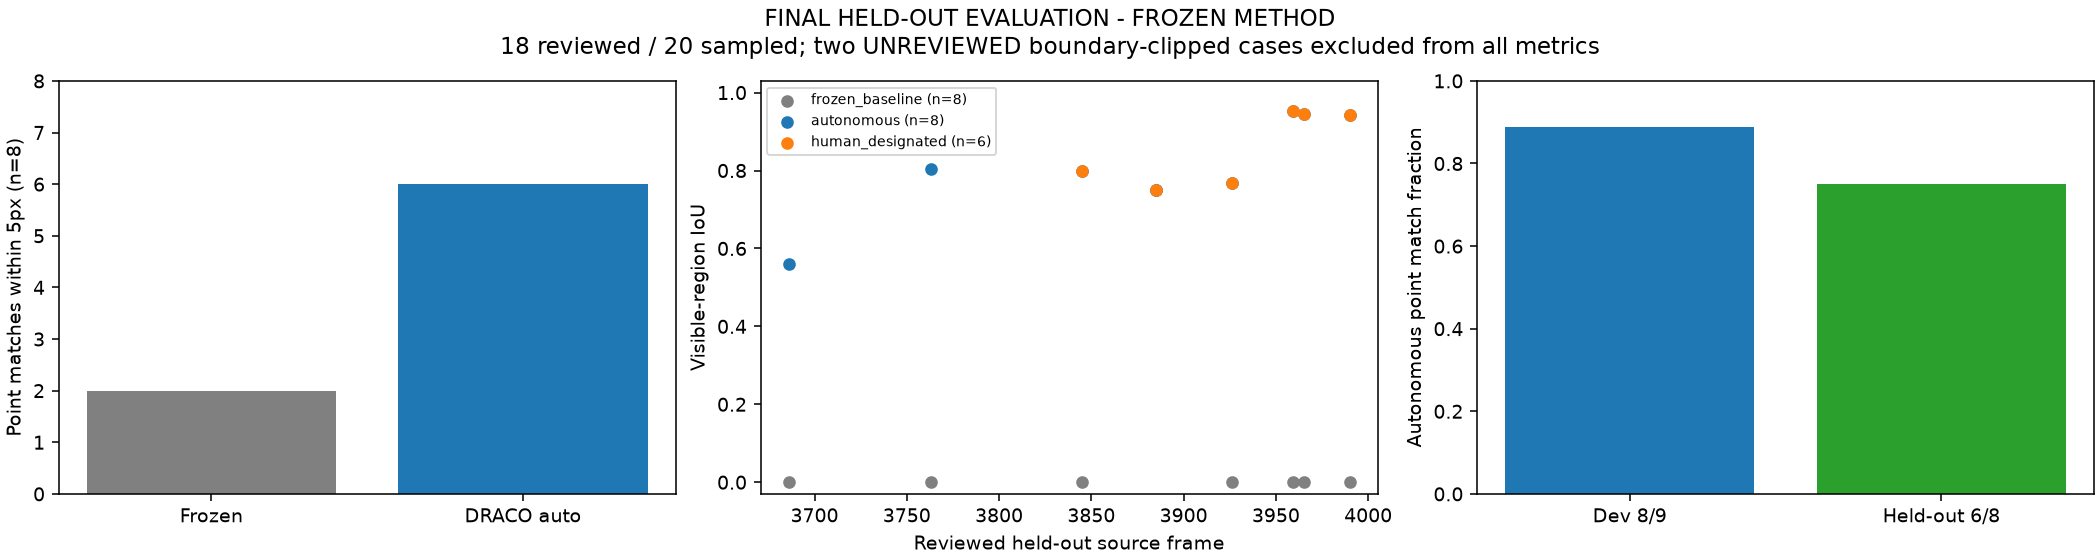
\includegraphics[width=\linewidth]{images/draco_heldout_benchmark.png}
\caption{Final held-out benchmark. Small samples, two excluded unreviewed boundary cases and absent reviewed final-ten-second coverage limit interpretation.}\label{fig:heldout}
\end{figure}
\section{AWS implementation and judge interaction}
The existing architecture is judge browser $\rightarrow$ EC2 $\rightarrow$ Nginx $\rightarrow$ Gunicorn $\rightarrow$ Flask $\rightarrow$ OpenDART/OpenCV~5 (Figure~\ref{fig:system}). A single CloudFormation-managed \texttt{c7i-flex.large} in \texttt{ap-southeast-2} runs Ubuntu 24.04 x86\_64, Python 3.12.3, OpenCV runtime 5.0.0 and \texttt{opencv-python==5.0.0.93}. The deployment uses an existing private encrypted S3 release/evidence bucket and Systems Manager administration; there is no added load balancer, GPU, second instance or container platform.

The public synthetic endpoint is \url{http://ec2-54-253-67-121.ap-southeast-2.compute.amazonaws.com/}. Four fixed presets execute the unchanged workload: NOMINAL and BLACKOUT reach TARGET\_IMPACT; NO\_MEASUREMENT and BALLISTIC return MISS. Latest recorded cloud runs took 13.79--14.16~s; earlier deployment measurements were approximately 14.1--14.5~s. All four numerical regression comparisons passed. Simulation runs are accelerated computation, not real-time mission control.

The separate \texttt{/draco} page provides 12 original calibrated PNGs, compact metadata, recorded replay, frozen benchmark/comparison figures and genuine live selected-frame inference. The curated bundle is 4.74~MB; neither the complete dataset, FITS nor XML corpus is uploaded. The browser-compatible replay is a presentation-only H.264 copy retaining all 4000 frames and 60~fps timing, approximately 66.667~s; inference was not regenerated for that transcode.

Figure~\ref{fig:aws} shows a live result. Every live DRACO request verifies hashes, restores validated past-only state saved immediately \emph{before} the chosen historical image, and then processes that original image afresh on EC2 with the unchanged frozen Features/Track methods. This checkpoint continuation preserves temporal semantics without replaying the complete prefix on every click. No current-frame target label is supplied, and no stored overlay substitutes for inference. All 12 continuations matched pre-existing frozen chronological predictions, locally and on Linux. Verified states include SEARCH\_UNRESOLVED, TRACKING, RESOLVED\_BODY and PARTIAL\_FRAME, with representative server processing approximately 118--130~ms. Request/subprocess overhead is additional.

\begin{figure}[htbp]\centering
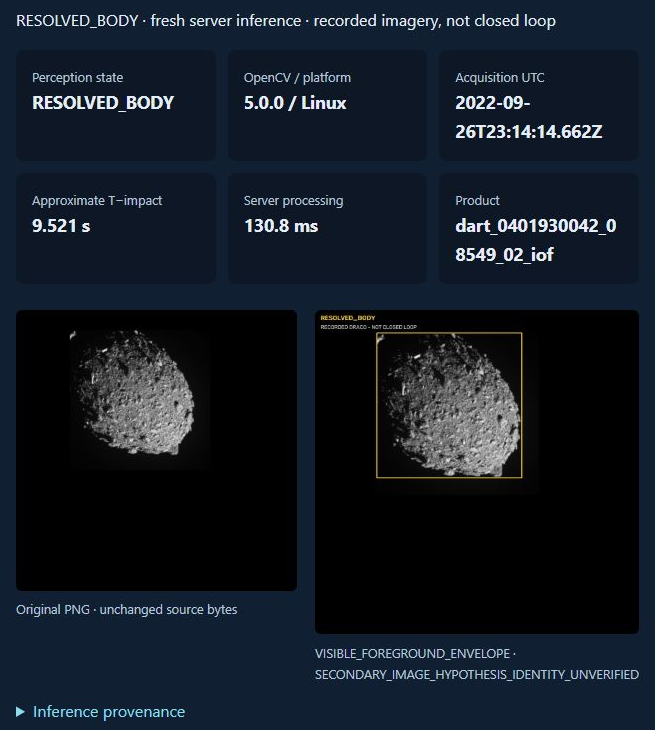
\includegraphics[width=.58\linewidth]{images/aws_live_resolved_detail.png}
\caption{Detail of the EC2 result: fresh OpenCV 5.0.0 inference and a coarse visible-region overlay. Historical imagery remains explicitly labelled as not closed loop.}\label{fig:aws}
\end{figure}

The website accepts fixed preset/image IDs, not arbitrary uploads, paths, URLs or scientific parameters. A global computation lock, request/rate limits, subprocess timeouts and 3~GiB application memory ceiling bound public use. The process-local hourly cap resets on restart. The public demonstration is HTTP without authentication/TLS and accepts only public inputs; it is not a hardened general-purpose service. Resource identities remained unchanged after the application-only release. CloudFormation bootstrap parameters retain the earlier release; recreating an instance requires reapplying the desired audited application update.

\section{Limitations, responsible use and reproducibility}
The main visual scenario is a bounded synthetic planar model with known target size, prescribed binary ephemeris, simplified illumination/shape/actuation, known camera geometry and idealised attitude knowledge. A reference image textures modelled geometry; it does not recover the historical trajectory. The 3D bearing experiments, planar visual system and real-image perception benchmark are separate evidence categories. No monocular range or physical centre is inferred from a DRACO visible-region box.

Covariance undercoverage prevents a statistical EKF-consistency claim. Size-prior diagnostics expose significant scale sensitivity even when contact succeeds. Ninety-six guided synthetic contacts do not establish broad reliability or flight readiness. The small reviewed real-image sample excludes two unreviewed boundary cases and provides no reviewed labels in the final ten seconds. Neither imagery replay nor browser inference validates real guidance. No crater, ejecta, deflection or post-contact dynamics model is implemented.

User interaction is deliberately constrained. Judges select fixed public presets; the synthetic guidance is autonomous after perception/estimation. Optional one-time operator designation exists only in recorded DRACO replay, not the live autonomous analyser or synthetic guidance. Telemetry and honest no-selection/hold/partial states expose limitations rather than conceal them.

The accompanying package contains pinned Python 3.12 dependencies, full core source/tests, exact build/test/deploy/cleanup instructions, selected frozen summaries and figure provenance, diagrams and report source. The core synthetic demonstration needs no DRACO download. Curated checkpoint inference is reproducible without the full archive; complete source-prefix reconstruction and independent annotation review require the original dataset/review inputs and are not claimed from the compact bundle alone. The one-shot held-out evaluation is preserved and was not rerun. Source/configuration and original-data hashes accompany the reproducibility material.

\section{Conclusion}
OpenDART delivers an inspectable OpenCV~5 perception--estimation--action loop whose applied commands change later synthetic images, with controlled AWS execution and matched negative controls. Separate frozen DRACO perception supplies a small, carefully delimited real-image benchmark. Its contribution is transparent integration and measurable behaviour under stated conditions, with uncertainty, observability, failures and responsible-use limits retained alongside successful outcomes.
\begin{thebibliography}{9}
\bibitem{gabern} F. Gabern, W. S. Koon and J. E. Marsden, ``Spacecraft Dynamics Near a Binary Asteroid,'' \emph{Discrete and Continuous Dynamical Systems}, Supplement, 2005, pp. 297--306.
\bibitem{voyatzis} G. Voyatzis, D. Karydis, I. Gkolias, M. Gaitanas and K. Tsiganis, ``Planar spacecraft trajectories in the Didymos--Dimorphos binary asteroid system,'' \emph{Planetary and Space Science}, 240, 105825, 2024.
\bibitem{atchison} J. A. Atchison, M. T. Ozimek, B. L. Kantsiper and A. F. Cheng, ``Trajectory options for the DART mission,'' \emph{Acta Astronautica}, 123, pp. 330--339, 2016.
\bibitem{bigot} J. Bigot et al., ``The bearing capacity of asteroid (65803) Didymos estimated from boulder tracks,'' \emph{Nature Communications}, 15, 6204, 2024.
\bibitem{ernst} C. M. Ernst et al., ``Calibration and In-flight Performance of DART's Didymos Reconnaissance and Asteroid Camera for OpNav (DRACO),'' \emph{The Planetary Science Journal}, 5, 257, 2024.
\bibitem{pds} PDS Small Bodies Node, calibrated DRACO v3.0 \texttt{data\_dracocal}, terminal/final collections, 2022/269. \url{https://pds-smallbodies.astro.umd.edu/holdings/pds4-dart:data_dracocal-v3.0/}.
\end{thebibliography}

\end{document}
